\section{Verhalten}
\subsection{}

\begin{frame}
    \frametitle{Technische Hilfsmittel}
    \begin{itemize}
        \item Browser-Plugin "HTTPS Everywhere" (eff.org/https-everywhere)
        \item Browser-Plugin "Disconnect.me" (disconnect.me)
        \item GPG (gnupg.org)
        \item Tor (torproject.org)
        \item Redphone (whispersystems.org)
        \item TextSecure (whispersystems.org)
    \end{itemize}
\end{frame}

\begin{frame}
    \frametitle{Datensparsamkeit}
    \begin{itemize}
        \item<2-> Viele Daten zusammen ergeben Profile
        \item<3-> Werden die Daten gebraucht?
        \item<4-> Werden echte Daten gebraucht?
            \begin{itemize}
              \item<5-> Pseudonymität
              \item<6-> mailinator.com (Wegwerf-Email-Adresse)
	      \item<7-> frank-geht-ran.de (Wegwerf-Telefonnummer)
              \item<8-> bugmenot.com (Fake Accounts)
            \end{itemize}
    \end{itemize}
\end{frame}

\begin{frame}
    \frametitle{Passwörter}
    \begin{itemize}
        \item<2-> Keine einfachen Wörter
        \item<3-> Groß-, Kleinbuchstaben, Ziffern, Sonderzeichen
        \item<4-> Beispiele:
            \begin{itemize}
                \item<5-> dragon
                \item<6-> (nCuAj.§Tsm!f
                \item<7-> IchLiebeDich
                \item<8-> .§)=")=`
                \item<10-> qwerty
                \item<11-> Mks?o/.u,1Psw!
            \end{itemize}
        \item<12-> Verschiedene Passwörter nutzen!
        \item<13-> Passwort-Manager verwenden \\ (z.B. Keepass, Password Safe)
    \end{itemize}
\end{frame}

\begin{frame}
    \frametitle{Wie schütze ich meinen Computer?}
    \begin{itemize}
      \item Firewall
      \item Aktuelle und vertrauenswürdige Software
    \end{itemize}
\end{frame}

\begin{frame}
    \frametitle{Wie schütze ich mein Smartphone?}
    \begin{itemize}
      \item Permissions
      \item Firewall (z.B. AFwall+)
      \item Aktuelle und vertrauenswürdige Software
      \item Alternativer Appstore: f-droid.org
    \end{itemize}
\end{frame}

\begin{frame}
    \frametitle{Freie Software}
    \begin{itemize}
      \item Firefox
      \item Thunderbird
      \item LibreOffice
      \item Pidgin
      \item Evince/Okular
      \item Gimp
      \item VLC
    \end{itemize}
\end{frame}

\begin{frame}
    \frametitle{Freie Software}
    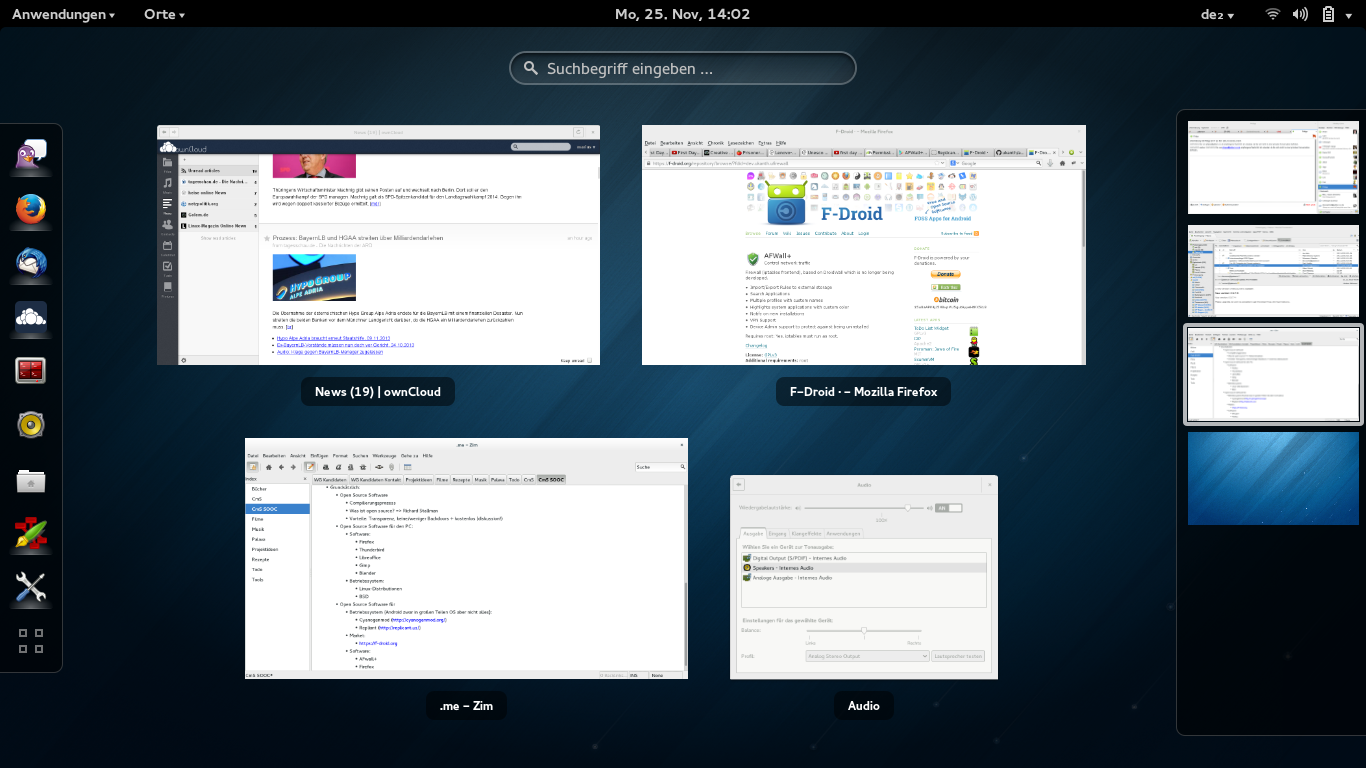
\includegraphics[height=0.7\textheight]{img/gnome.png}
\end{frame}

\begin{frame}
    \frametitle{Freie Software}
    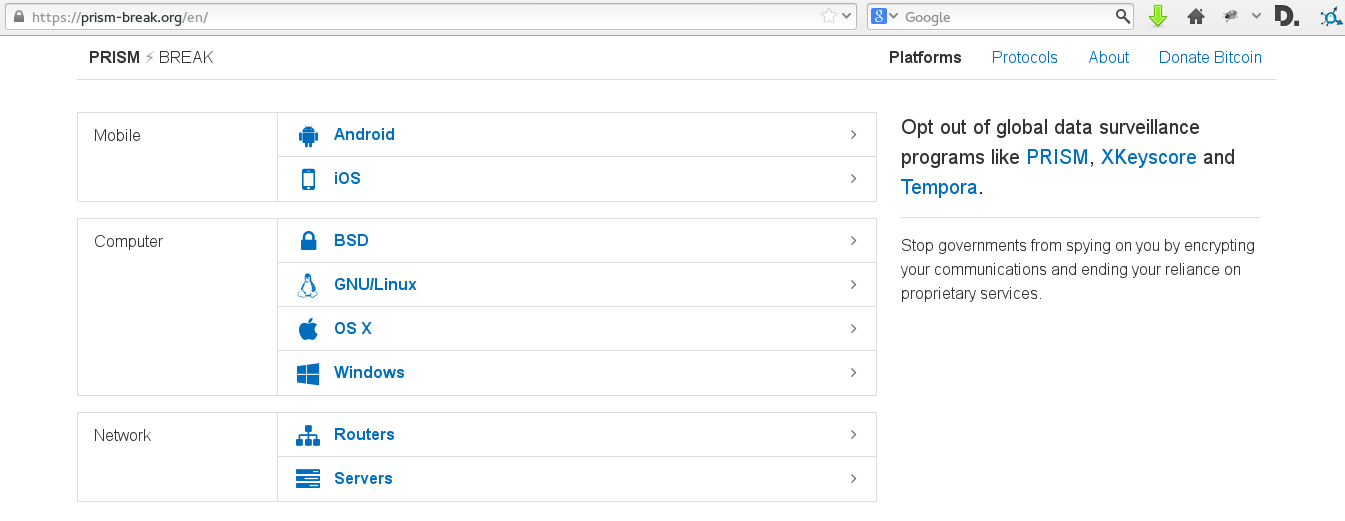
\includegraphics[height=0.7\textheight]{img/prism-break1.png}
\end{frame}

\begin{frame}
    \frametitle{Freie Software}
    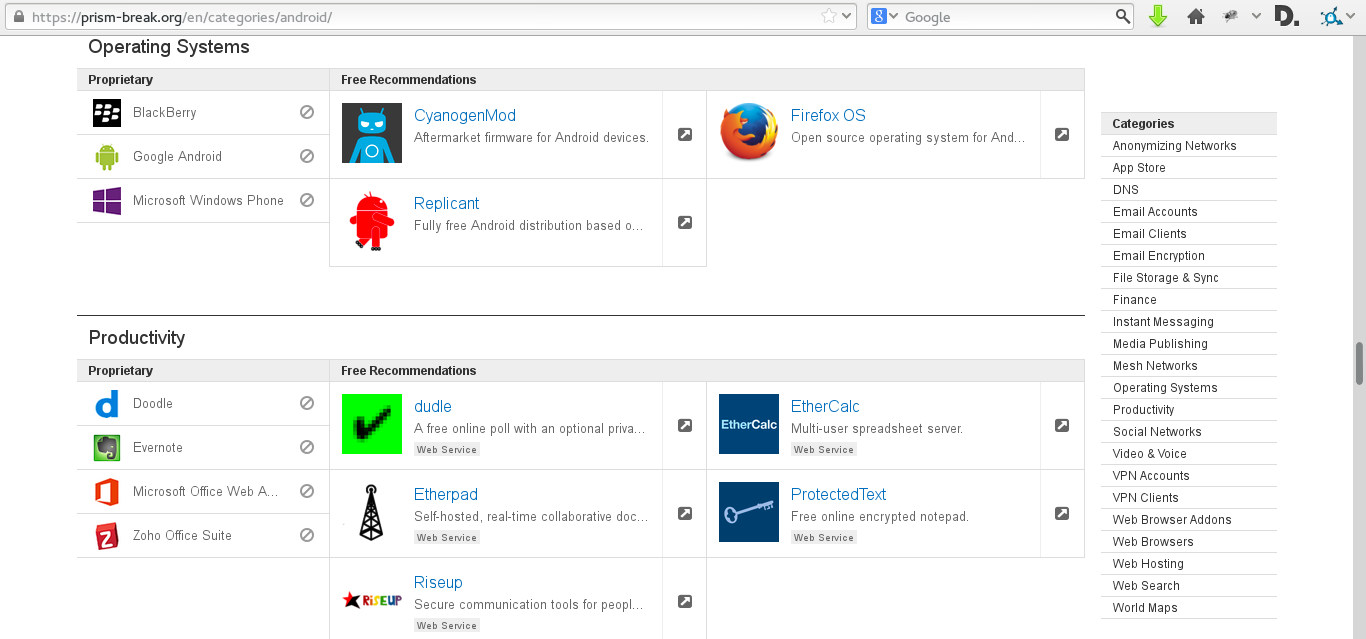
\includegraphics[height=0.7\textheight]{img/prism-break2.png}
\end{frame}

\begin{frame}
    \frametitle{Diskussion}
    \begin{center} {\Large Diskussion}\\Marius Melzer und Stephan Thamm\\CMS Dresden: schule@c3d2.de, c3d2.de/schule.html \end{center}
    \begin{center}
      \href{https://creativecommons.org/licenses/by-sa/4.0/}{\cc{by-sa}} \\
      \href{https://github.com/c3d2/cms/tree/master/2014_03_25_bischofswerda}{\textcolor{blue}{Folien}} vom Chaos Computer Club Dresden
    \end{center}
\end{frame}

\begin{frame}
    \frametitle{Weiterführende Links}
    \begin{itemize}
        \item Überwachungsstaat, was ist das? - \url{https://www.youtube.com/watch?v=iHlzsURb0WI}
        \item Übersicht freier PDF-Betrachter - \url{http://pdfreaders.org}
        \item Freie Alternativen zu kommerzieller Software - \url{http://prism-break.org}
        \item Übersicht öffentlicher Jabber-Server - \url{https://xmpp.net/directory.php}
    \end{itemize}
\end{frame}